\section{Motivation and Challenges}\label{sec:motivation}


In this section, we will discuss the importance of taking model interference into account when inference serving, as demonstrated by the suboptimal performance of existing approaches.

\begin{figure}
	\centering
	\begin{subfigure}[t]{0.45\textwidth}
		\centering
		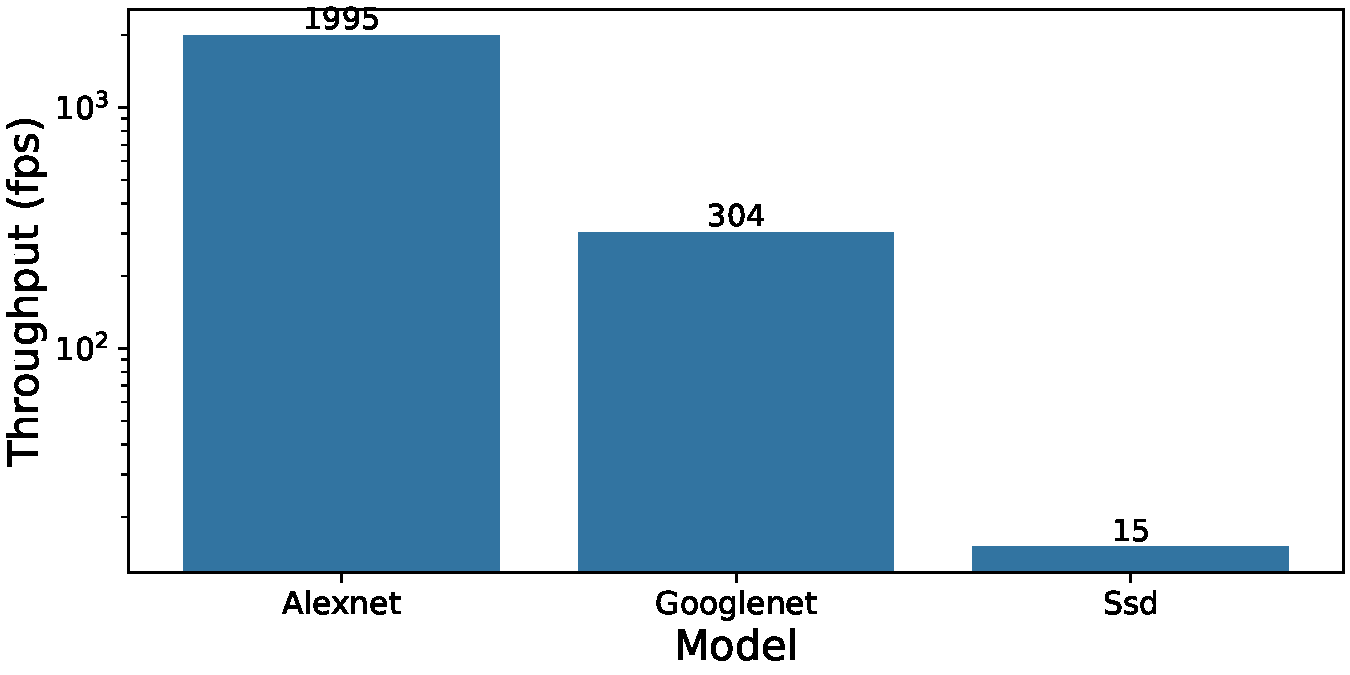
\includegraphics[width=\textwidth]{chapters/roomie/images/Throughput_models_in_isolation.pdf}
		\caption{Throughput when the model operates in isolation, without any interference.}
		\label{fig:isolation}
	\end{subfigure}
	\hfill
	\begin{subfigure}[t]{0.45\textwidth}
		\centering
		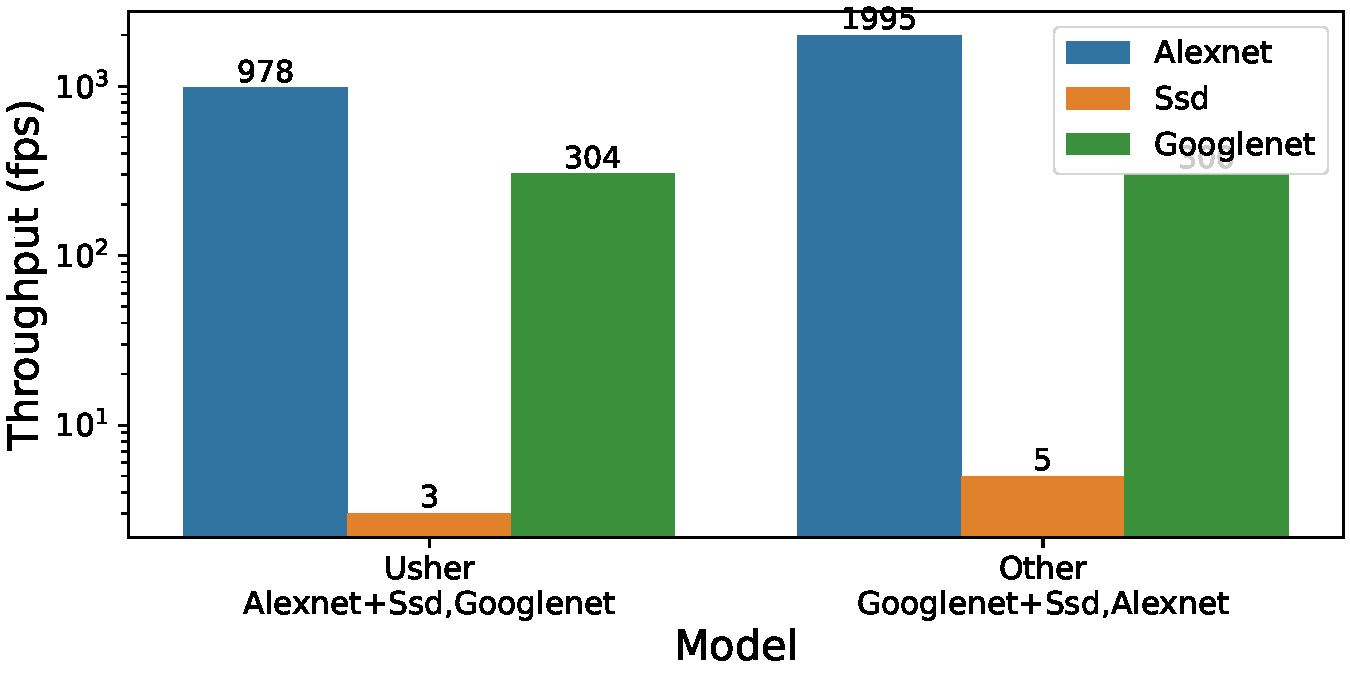
\includegraphics[width=\textwidth]{chapters/roomie/images/Throughput_models_in_combinaison.pdf}
		\caption{An alternative to co-locating three models on two GPUs, offering a better compromise than Usher~\cite{shubha2024usher}.}
		\label{fig:colocation}
	\end{subfigure}
	\label{fig:three graphs}
\end{figure}

\subsection{Limitations of Existing Inference Serving Strategies}

The deployment of machine learning models for inference serving has become increasingly critical across domains such as computer vision, natural language processing, and recommendation systems. As demand for real-time inference grows, organizations are compelled to maximize the utilization of existing computational infrastructure, particularly in resource-constrained environments. While scalable serving architectures have been proposed to meet service level objectives (SLOs), such as latency and throughput, many existing systems rely on simplistic heuristics for model placement and colocation. These approaches typically reference offline profiling data or prioritize devices with the most available memory, overlooking the nuanced performance degradation that arises when multiple models share GPU resources.

The assumption that memory availability is a reliable proxy for inference performance is mistaken. During inference, models consume significantly less memory compared to training, as intermediate states and gradients are not retained. Consequently, memory-centric placement decisions fail to account for the dynamic interference between concurrently executing models. Systems such as Usher attempt to address this by analyzing low-level GPU kernels to estimate resource demands. However, their methodology does not capture the complex interactions between kernels from different models, leading to suboptimal colocation choices.

We conducted an experimental study to evaluate the performance of three inference models: AlexNet, GoogLeNet, and SSD, on two Jetson Xavier devices. The performance of each deep neural network (DNN) when operating in isolation is illustrated in~\Cref{fig:isolation}. Our primary objective was to identify the optimal co-location configuration among all possible combinations. Our findings revealed that Usher's proposed approach of co-locating AlexNet with SSD is not necessarily the most effective option. In fact, an alternative configuration, GoogLeNet paired with SSD—demonstrates a superior balance in performance (refer to Figure colocation).

We have determined that Usher's misjudgment stems from the method used to assess model compatibility. Merely classifying models based on their computing or memory capacity does not provide a comprehensive understanding of their performance. A more nuanced approach that considers the resource demands of each model over time is essential for accurate evaluation.


\subsection{The Importance of Kernel-Level Analysis}

Deep neural networks (DNNs) perform inference by executing a sequence of GPU kernels, each responsible for specific low-level computations and defined by distinct resource requirements such as shared memory, register usage, and execution time. These kernels, rather than the high-level model architecture, constitute the true computational footprint on the GPU. Profiling tools such as Nsight Systems~\cite{nsight_systems} and Torch Profiler~\cite{torch_profiler} enable fine-grained observation of kernel behavior, revealing patterns of resource occupancy and execution timing that are often obscured at the model level. Empirical analysis shows that individual kernels frequently leave portions of the GPU underutilized, suggesting that with careful orchestration, multiple models can be deployed simultaneously to improve overall throughput.

However, when models are executed concurrently on the same GPU, their kernels may overlap in time and compete for limited hardware resources. Although this parallelism can enhance utilization, it also introduces a critical challenge: interference. This occurs when the combined resource demands of overlapping kernels exceed the GPU's capacity, forcing the hardware to serialize execution or delay kernel launches. For instance, if two kernels simultaneously require more shared memory or registers than the GPU can allocate, contention arises, leading to extended execution times and degraded performance. The severity of interference is shaped not only by the type of resources consumed but also by the duration and temporal alignment of kernel execution. Without precise modeling of these interactions, colocation decisions risk undermining system efficiency rather than enhancing it.

Effective colocation requires more than simply identifying underutilized resources; it demands a precise understanding of how kernels from different models interact during concurrent execution. The configuration of each kernel (its use of shared memory, registers, and other architectural resources) determines its potential for interference with others. Predicting these interferences cannot be based solely on aggregated model statistics or layer-level abstractions, as these overlook the fine-grained execution dynamics that govern actual performance. Instead, kernel-level analysis must consider both static resource requirements and temporal execution behavior to assess how overlapping workloads compete for limited GPU capacity. By modeling these interactions, it becomes possible to identify model pairs that minimize conflicts and make informed colocation decisions that preserve throughput and latency under constrained conditions.

\subsection{Challenges in Modeling and Predicting Interference}

% \begin{figure}
% 	\centering
% 	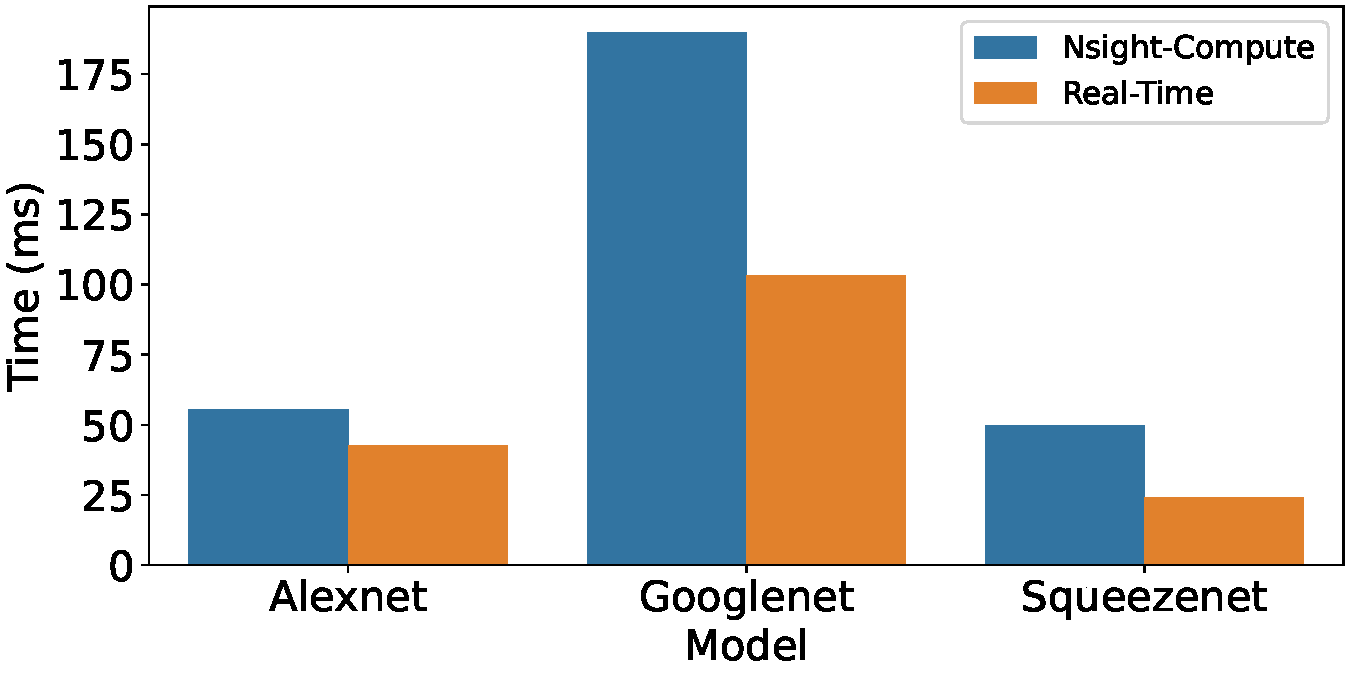
\includegraphics[width=\textwidth]{chapters/roomie/images/duration_gap.pdf}
% 	\caption{Throughput when the model operates in isolation, without any interference.}
% 	\label{fig:duration_gap}
% \end{figure}

Determining the best colocation strategy for deep neural networks (DNNs) sharing a GPU requires a nuanced understanding of how their kernels interact during inference. The goal is to identify model pairings that maximize throughput and minimize latency by avoiding harmful interference. Achieving this demands accurate performance modeling at the kernel level, where resource contention and execution overlap directly impact runtime behavior. However, building such models introduces several practical and computational challenges that must be addressed to ensure scalability and reliability.

\paragraph{Profiling overhead and trace collection.}
% Profiling is essential for capturing the fine-grained execution characteristics of DNN kernels, including resource usage and execution time. These metrics form the backbone of any interference-aware colocation strategy. Yet, collecting accurate traces is inherently time-consuming and introduces overhead that can distort the very measurements it seeks to record. Profiling tools rely on instrumentation and callbacks that add latency to kernel execution, often resulting in total recorded durations that exceed the actual inference time. This discrepancy complicates performance estimation and can mislead scheduling decisions if left uncorrected. Despite these limitations, profiling remains indispensable, as predicting kernel behavior analytically is highly challenging due to the variability in runtime configurations and hardware-specific optimizations. Fortunately, the process can be made tractable by profiling models in isolation. Since the number of GPU architectures in deployment is relatively small, and many models follow standardized execution patterns, it is feasible to build a reusable profiling database that supports accurate interference modeling without incurring prohibitive cost.
% Profiling is crucial for capturing the detailed execution characteristics of Deep Neural Network (DNN) kernels, particularly regarding resource usage and execution time, which are essential for interference-aware colocation strategies. However, the process of collecting accurate execution traces is time-consuming and introduces overhead that can distort measurements, often resulting in recorded durations that exceed actual inference times. This discrepancy complicates performance estimation and may mislead scheduling decisions if uncorrected. Despite these limitations, profiling is indispensable, as predicting kernel behavior analytically is challenging due to variability in runtime configurations and hardware-specific optimizations. Profiling models in isolation can alleviate some of these issues, and given the relatively small number of GPU architectures in use and the standardized execution patterns of many models, it is feasible to create a reusable profiling database that supports accurate interference modeling without incurring prohibitive costs.
Profiling is essential for capturing the fine-grained execution characteristics of DNN kernels, including resource occupancy and duration. These metrics form the backbone of any interference-aware colocation strategy. Yet, collecting accurate traces is inherently time-consuming and introduces overhead that can distort the very measurements it seeks to record. Profiling tools rely on instrumentation and callbacks that add latency to kernel execution, often resulting in total recorded durations that exceed the actual inference time.
In practice, we observed that the ratio between profiled kernel durations and actual inference time can vary considerably, sometimes exceeding the true runtime by a wide margin, highlighting how profiling overhead may distort performance measurements and must be carefully considered.
% This discrepancy complicates performance estimation and can mislead scheduling decisions. Figure~\ref{fig:duration_gap} illustrates this phenomenon, showing the gap between the measured inference time and the aggregate kernel durations.
Despite these limitations, profiling remains indispensable, as predicting kernel behavior analytically is highly challenging due to the variability in runtime configurations and hardware-specific optimizations. What's more, cuDNN~\cite{cudnn} provides highly tuned implementations for standard routines such as convolution, attention, matrix multiplication, pooling, and normalization. For the same operator type, it may execute different kernels depending on the GPU architecture and available resources, with varying configurations in register usage, shared memory, and execution strategy. While this process is time-consuming, it remains feasible due to the limited number of GPU variants and the ability to profile models only in isolation.

\paragraph{Combinatorial Complexity of Kernel Overlap Scenarios.}
% Another significant challenge lies in modeling the overlapping execution of kernels across multiple DNN models. While the analytical framework developed earlier enables estimation of interference effects, applying it exhaustively is computationally prohibitive. Real-world deployments do not guarantee synchronized kernel execution; instead, each model may begin inference from any point in its kernel sequence. Evaluating all possible alignments requires constructing a full Cartesian product of starting indices, resulting in exponential growth in the number of scenarios as the number of models increases. This combinatorial explosion makes real-time evaluation impractical.
A key challenge in optimizing deep neural network colocation lies in defining and identifying the interference itself. Interference is not a static property: it arises dynamically when the kernels of different models overlap during execution and compete for shared GPU resources. To determine which kernels are likely to interfere, it is necessary to analyze not only their resource requirements, but also their temporal alignment and execution context. This is particularly difficult because interference depends on both the type and timing of resource usage, which can vary across deployments and hardware configurations.\\
This challenge is compounded by the vast number of possible overlapping scenarios. In realistic service environments, models do not begin inference in a synchronized manner; each can start at any point in its kernel sequence, leading to a vast space of potential execution alignments. Taking into account all combinations of starting positions across multiple models leads to exponential growth in the number of scenarios as the number of models increases. This combinatorial explosion makes exhaustive evaluation impractical for real-time decision-making. The challenge lies in estimating the impact of interference without simulating all possible alignments, while maintaining sufficient fidelity to guide effective colocation strategies.

To support efficient colocation of deep neural networks on shared GPUs, we introduce~\roomie, a kernel-level profiling and interference estimation strategy that balances precision with scalability. By analyzing execution traces in isolation and simulating representative overlap scenarios,~\roomie{} enables informed deployment decisions without incurring prohibitive computational cost.



% Modeling kernel interference presents several challenges. First, the diversity of GPU architectures and model types necessitates extensive offline profiling to capture performance characteristics across deployment scenarios. While this process is time-consuming, it remains feasible due to the limited number of GPU variants and the ability to profile models in isolation. Second, predicting interference requires identifying which kernels will overlap in execution and assessing the impact on their runtime. This involves analyzing resource contention at a granular level, including shared memory and register usage, and determining whether the combined demand exceeds the GPU's capacity.

% Furthermore, the execution order of kernels and their serialization within CUDA streams influence the degree of interference. Kernels with complementary resource profiles may coexist with minimal performance degradation, while those with overlapping demands can significantly delay each other's execution. Existing approaches that rely solely on layer-level information or aggregate model statistics fail to capture these subtleties. Therefore, a more refined methodology is required—one that profiles kernels individually, models their interactions, and predicts the resulting performance impact under colocation. Addressing these challenges is essential for enabling efficient inference serving in environments where computational resources are limited and colocation is unavoidable.